\documentclass[]{article}
\usepackage{lmodern}
\usepackage{amssymb,amsmath}
\usepackage{ifxetex,ifluatex}
\usepackage{fixltx2e} % provides \textsubscript
\ifnum 0\ifxetex 1\fi\ifluatex 1\fi=0 % if pdftex
  \usepackage[T1]{fontenc}
  \usepackage[utf8]{inputenc}
\else % if luatex or xelatex
  \ifxetex
    \usepackage{mathspec}
  \else
    \usepackage{fontspec}
  \fi
  \defaultfontfeatures{Ligatures=TeX,Scale=MatchLowercase}
\fi
% use upquote if available, for straight quotes in verbatim environments
\IfFileExists{upquote.sty}{\usepackage{upquote}}{}
% use microtype if available
\IfFileExists{microtype.sty}{%
\usepackage{microtype}
\UseMicrotypeSet[protrusion]{basicmath} % disable protrusion for tt fonts
}{}
\usepackage[margin=1in]{geometry}
\usepackage{hyperref}
\hypersetup{unicode=true,
            pdftitle={Analysis of Tissue Weights from HFD/Dexamethasone Studies},
            pdfauthor={Innocence Harvey and Dave Bridges},
            pdfborder={0 0 0},
            breaklinks=true}
\urlstyle{same}  % don't use monospace font for urls
\usepackage{longtable,booktabs}
\usepackage{graphicx,grffile}
\makeatletter
\def\maxwidth{\ifdim\Gin@nat@width>\linewidth\linewidth\else\Gin@nat@width\fi}
\def\maxheight{\ifdim\Gin@nat@height>\textheight\textheight\else\Gin@nat@height\fi}
\makeatother
% Scale images if necessary, so that they will not overflow the page
% margins by default, and it is still possible to overwrite the defaults
% using explicit options in \includegraphics[width, height, ...]{}
\setkeys{Gin}{width=\maxwidth,height=\maxheight,keepaspectratio}
\IfFileExists{parskip.sty}{%
\usepackage{parskip}
}{% else
\setlength{\parindent}{0pt}
\setlength{\parskip}{6pt plus 2pt minus 1pt}
}
\setlength{\emergencystretch}{3em}  % prevent overfull lines
\providecommand{\tightlist}{%
  \setlength{\itemsep}{0pt}\setlength{\parskip}{0pt}}
\setcounter{secnumdepth}{0}
% Redefines (sub)paragraphs to behave more like sections
\ifx\paragraph\undefined\else
\let\oldparagraph\paragraph
\renewcommand{\paragraph}[1]{\oldparagraph{#1}\mbox{}}
\fi
\ifx\subparagraph\undefined\else
\let\oldsubparagraph\subparagraph
\renewcommand{\subparagraph}[1]{\oldsubparagraph{#1}\mbox{}}
\fi

%%% Use protect on footnotes to avoid problems with footnotes in titles
\let\rmarkdownfootnote\footnote%
\def\footnote{\protect\rmarkdownfootnote}

%%% Change title format to be more compact
\usepackage{titling}

% Create subtitle command for use in maketitle
\newcommand{\subtitle}[1]{
  \posttitle{
    \begin{center}\large#1\end{center}
    }
}

\setlength{\droptitle}{-2em}
  \title{Analysis of Tissue Weights from HFD/Dexamethasone Studies}
  \pretitle{\vspace{\droptitle}\centering\huge}
  \posttitle{\par}
  \author{Innocence Harvey and Dave Bridges}
  \preauthor{\centering\large\emph}
  \postauthor{\par}
  \predate{\centering\large\emph}
  \postdate{\par}
  \date{April 7, 2017}


\begin{document}
\maketitle

{
\setcounter{tocdepth}{2}
\tableofcontents
}
\section{Data Entry}\label{data-entry}

This script generates figures from the tissue weights found in
../../data/raw/HFD and Chow Tissue Weights.csv. This file is located in
/Users/davebrid/Documents/GitHub/CushingAcromegalyStudy/scripts/scripts-obesity
and was most recently updated on Tue Aug 8 20:00:50 2017.

\section{Number of Animals}\label{number-of-animals}

\begin{longtable}[]{@{}lllr@{}}
\caption{Number of mice in each group}\tabularnewline
\toprule
Status & Diet & Treatment & Number\tabularnewline
\midrule
\endfirsthead
\toprule
Status & Diet & Treatment & Number\tabularnewline
\midrule
\endhead
Fasted & NCD & Water & 8\tabularnewline
Fasted & NCD & Dexamethasone & 8\tabularnewline
Fasted & HFD & Water & 22\tabularnewline
Fasted & HFD & Dexamethasone & 12\tabularnewline
Fed & NCD & Water & 4\tabularnewline
Fed & NCD & Dexamethasone & 4\tabularnewline
\bottomrule
\end{longtable}

\section{Summary Data}\label{summary-data}

The remainder of this analysis is only for Fasted animals

\begin{longtable}[]{@{}llrrrr@{}}
\caption{Averaged Values}\tabularnewline
\toprule
Diet & Treatment & iWAT\_mean.na & eWAT\_mean.na & TS\_mean.na &
Quad\_mean.na\tabularnewline
\midrule
\endfirsthead
\toprule
Diet & Treatment & iWAT\_mean.na & eWAT\_mean.na & TS\_mean.na &
Quad\_mean.na\tabularnewline
\midrule
\endhead
NCD & Water & 140.9750 & 187.1125 & 163.3750 & 240.0250\tabularnewline
NCD & Dexamethasone & 111.0625 & 173.1875 & 144.5000 &
197.8250\tabularnewline
HFD & Water & 840.7545 & 1136.3773 & 190.6905 & 241.7727\tabularnewline
HFD & Dexamethasone & 286.8000 & 464.1000 & 127.4417 &
139.5000\tabularnewline
\bottomrule
\end{longtable}

\section{Muscle Barplots}\label{muscle-barplots}

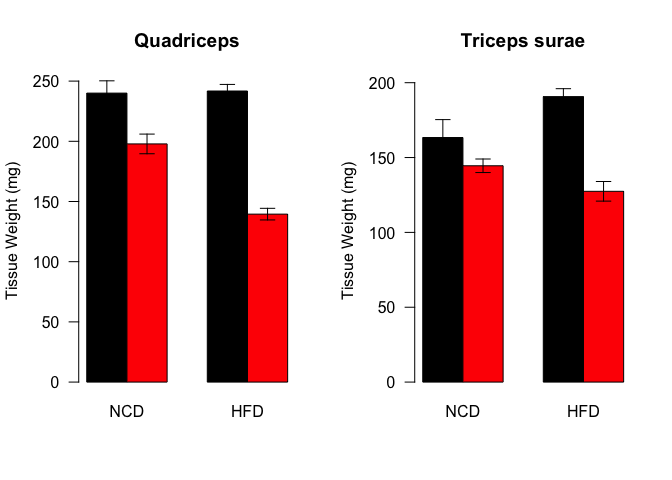
\includegraphics{figures/muscle-weight-barplot-1.png}

\section{Adipose Barplots}\label{adipose-barplots}

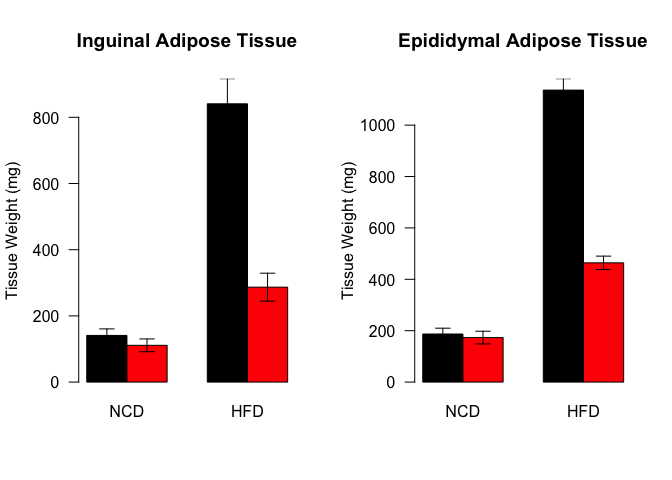
\includegraphics{figures/adipose-weight-barplot-1.png}

\subsection{Analysis of Adipose Tissue
Weights}\label{analysis-of-adipose-tissue-weights}

We observed reductions in both iWAT and eWAT with HFD/Dexamethasone.

\subsubsection{Inguinal Adipose Tissue}\label{inguinal-adipose-tissue}

This included a 65.8877848\% reduction in iWAT mass in the HFD mice. A
Shapiro-Wilk test of the iWAT values had a p-value of
\textgreater{}0.0621229, so normality could be assumed. To test for
equal variance, Levene's tests were performed.

The p-value from the Levene's test were 0.0041061 for HFD. Based on this
a Welch's \emph{t} test was performed with a p-value of
\textbf{4.4777019× 10\textsuperscript{-7}}.

For NCD the Levene's test had a p-value of and 0.2829918, so equal
variance could be assumed. Based on this, a Student's \emph{t}-test had
a p-value of \textbf{0.4967434} for NCD.

There was only a 21.2183011\% reduction in iWAT mass in the NCD mice.

Based on a 2-way ANOVA with Diet and Group as the interacting covariates
there was a significant interaction between diet and treatment:

\begin{longtable}[]{@{}lrrrrr@{}}
\caption{Two Way ANOVA with Interaction between treatment and
diet.}\tabularnewline
\toprule
term & df & sumsq & meansq & statistic & p.value\tabularnewline
\midrule
\endfirsthead
\toprule
term & df & sumsq & meansq & statistic & p.value\tabularnewline
\midrule
\endhead
Diet & 1 & 3579646.8 & 3579646.80 & 65.49123 & 0.00e+00\tabularnewline
Group & 1 & 1400297.4 & 1400297.44 & 25.61906 & 5.20e-06\tabularnewline
Diet:Group & 1 & 983744.2 & 983744.15 & 17.99804 &
8.73e-05\tabularnewline
Residuals & 54 & 2951554.4 & 54658.42 & NA & NA\tabularnewline
\bottomrule
\end{longtable}

The p-value for the interaction was \textbf{8.7281221×
10\textsuperscript{-5}}. The residuals of this model, passed through a
Shapiro-Wilk test had a p-value of 0.0015701, so normality could not be
assumed.

\subsubsection{Epididimal Adipose
Tissue}\label{epididimal-adipose-tissue}

This included a 59.1596901\% reduction in eWAT mass in the HFD mice.

There was only a 7.4420469\% reduction in eWAT mass in the NCD mice.

The p-value from the Levene's test were 0.0298476 for HFD. Based on this
a Welch's \emph{t} test was performed with a p-value of
\textbf{3.7377627× 10\textsuperscript{-14}}.

For NCD the Levene's test had a p-value of and 0.8965011, so equal
variance could be assumed. Based on this, a Student's \emph{t}-test had
a p-value of \textbf{0.5452112} for NCD.

Based on a 2-way ANOVA with Diet and Group as the interacting covariates
there was a significant interaction between diet and treatment:

\begin{longtable}[]{@{}lrrrrr@{}}
\caption{Two Way ANOVA with Interaction between treatment and
diet.}\tabularnewline
\toprule
term & df & sumsq & meansq & statistic & p.value\tabularnewline
\midrule
\endfirsthead
\toprule
term & df & sumsq & meansq & statistic & p.value\tabularnewline
\midrule
\endhead
Diet & 1 & 6924250 & 6924250.12 & 342.62891 & 0\tabularnewline
Group & 1 & 2055412 & 2055411.62 & 101.70682 & 0\tabularnewline
Diet:Group & 1 & 1455533 & 1455532.97 & 72.02335 & 0\tabularnewline
Residuals & 54 & 1091296 & 20209.18 & NA & NA\tabularnewline
\bottomrule
\end{longtable}

The p-value for the interaction was \textbf{1.6294353×
10\textsuperscript{-11}}. The residuals of this model, passed through a
Shapiro-Wilk test had a p-value of 0.0049698, so normality could not be
assumed.

\section{Session Information}\label{session-information}

\begin{verbatim}
## R version 3.3.0 (2016-05-03)
## Platform: x86_64-apple-darwin13.4.0 (64-bit)
## Running under: OS X 10.12.6 (unknown)
## 
## locale:
## [1] en_US.UTF-8/en_US.UTF-8/en_US.UTF-8/C/en_US.UTF-8/en_US.UTF-8
## 
## attached base packages:
## [1] stats     graphics  grDevices utils     datasets  methods   base     
## 
## other attached packages:
## [1] broom_0.4.2   car_2.1-4     forcats_0.2.0 readr_1.1.0   dplyr_0.5.0  
## [6] tidyr_0.6.1   knitr_1.15.1 
## 
## loaded via a namespace (and not attached):
##  [1] Rcpp_0.12.10       nloptr_1.0.4       highr_0.6         
##  [4] plyr_1.8.4         tools_3.3.0        digest_0.6.12     
##  [7] lme4_1.1-12        evaluate_0.10      tibble_1.3.0      
## [10] nlme_3.1-131       lattice_0.20-35    mgcv_1.8-17       
## [13] Matrix_1.2-8       psych_1.7.3.21     DBI_0.6-1         
## [16] yaml_2.1.14        parallel_3.3.0     SparseM_1.76      
## [19] stringr_1.2.0      MatrixModels_0.4-1 hms_0.3           
## [22] rprojroot_1.2      nnet_7.3-12        grid_3.3.0        
## [25] R6_2.2.0           foreign_0.8-67     rmarkdown_1.6     
## [28] minqa_1.2.4        reshape2_1.4.2     magrittr_1.5      
## [31] backports_1.0.5    htmltools_0.3.5    MASS_7.3-45       
## [34] splines_3.3.0      assertthat_0.1     pbkrtest_0.4-7    
## [37] mnormt_1.5-5       quantreg_5.29      stringi_1.1.3     
## [40] lazyeval_0.2.0
\end{verbatim}


\end{document}
